\documentclass[aspectratio=169,11pt]{ctexbeamer}

\usepackage[T1]{fontenc}
\usepackage{amsmath,amssymb}
\usepackage{booktabs}
\usepackage{listings}
\usepackage{xcolor}
\usepackage{hyperref}

\usepackage{xmum_beamer}

\title[厦门大学马来西亚分校深蓝主题风格 Beamer 模板使用说明]{厦门大学马来西亚分校\\深蓝主题风格 Beamer 模板使用说明}
\subtitle{Deep Blue Theme Beamer Template User Guide}
\author[zeyu10]{\texorpdfstring{作者：\href{mailto:zeyu1024@outlook.com}{崔泽禹}\\\url{https://github.com/zeyu10/xmum-beamer-template}}{作者：崔泽禹}}
\institute[SCDS | XMUM]{School of Computing and Data Science, Xiamen University Malaysia}
\date{\today}

\lstset{
    language=C++,
    basicstyle=\ttfamily\small,
    keywordstyle=\color{xmumblue}\bfseries,
    commentstyle=\color{green!45!black},
    stringstyle=\color{orange!70!black},
    showstringspaces=false,
    breaklines=true,
    frame=single
}

\begin{document}

\XMUMSetLogoPath{logo}
\XMUMSetBackgroundImage{xmum_building_blue.png}
\XMUMSetBackgroundOpacity{0.10}

% \XMUMSetLanguageChinese                                 % 语言设置方式1：中文（默认）
% \XMUMSetLanguageEnglish                                 % 语言设置方式2：英文

% \XMUMSetBackgroundBoth                                  % 背景设置方式1：标题页和帧均开启（默认）
% \XMUMSetBackgroundTitleOnly                             % 背景设置方式2：只开启标题页背景
% \XMUMSetBackgroundTitleAndToc                           % 背景设置方式3：只开启标题页和目录页背景
% \XMUMSetBackgroundFrameOnly                             % 背景设置方式4：只开启帧背景
% \XMUMSetBackgroundNone                                  % 背景设置方式5：都不开启背景
% \begin{frame}[nobg]{本页关闭背景}                        % 单页背景设置：默认有背景，添加 nobg 可关闭当前页背景
% \end{frame}

% \XMUMSetNavigationOff                                   % 导航按键设置方式1：关闭（默认）
% \XMUMSetNavigationOn                                    % 导航按键设置方式2：在右下角显示

% \XMUMSetTitleLogoDefault                                % 主标题页上方logo方式1：默认（带文字长版校徽）
% \XMUMSetTitleLogoNone                                   % 主标题页上方logo方式2：不显示任何logo
% \XMUMSetTitleLogoPure                                   % 主标题页上方logo方式3：校徽（无文字圆形校徽）
% \XMUMSetTitleLogo{logo_01}                              % 主标题页上方logo方式4：单个自定义logo
% \XMUMSetTitleLogo{logo_01.png,logo_02.png,logo_03.png}  % 主标题页上方logo方式4：多个自定义logo

% \XMUMSetFrameLogoDefault                                % 帧标题栏右侧logo方式1：默认（带文字长版校徽）
% \XMUMSetFrameLogoNone                                   % 帧标题栏右侧logo方式2：不显示任何logo
% \XMUMSetFrameLogoPure                                   % 帧标题栏右侧logo方式3：校徽（无文字圆形校徽）
% \XMUMSetFrameLogo{logo_01}                              % 帧标题栏右侧logo方式4：单个自定义logo
% \XMUMSetFrameLogo{logo_01.png,logo_02.png,logo_03.png}  % 帧标题栏右侧logo方式4：多个自定义logo

\XMUMTitleFrame

\begin{frame}{目录}
    \tableofcontents
\end{frame}

\section{编译说明}

\begin{frame}{如何编译}
    \begin{itemize}
        \item 若文档中没有额外调用 \texttt{.bib} 文献库文件，使用 \texttt{XeLaTeX} 连续编译两次即可。
        \item 若文档中调用了额外的 \texttt{.bib} 文献库文件，则需按照 \texttt{XeLaTeX} $\to$ \texttt{BibTeX} $\to$ \texttt{XeLaTeX} $\to$ \texttt{XeLaTeX} 的顺序编译。
    \end{itemize}

    \begin{exampleblock}{无额外参考文献时}
        \texttt{xelatex xmum\_beamer\_readme.tex}\\
        \texttt{xelatex xmum\_beamer\_readme.tex}
    \end{exampleblock}

    \begin{exampleblock}{含 \texttt{.bib} 文件时}
        \texttt{xelatex xmum\_beamer\_readme.tex}\\
        \texttt{bibtex xmum\_beamer\_readme}\\
        \texttt{xelatex xmum\_beamer\_readme.tex}\\
        \texttt{xelatex xmum\_beamer\_readme.tex}
    \end{exampleblock}
\end{frame}

\begin{frame}{如何编译}
    \begin{itemize}
        \item 或使用集成开发环境（如 \href{https://texstudio.sourceforge.net}{TeXstudio}、\href{https://www.overleaf.com/project}{Overleaf}）进行编译。
        \item 也可在 VS Code 中使用 \href{https://marketplace.visualstudio.com/items?itemName=James-Yu.latex-workshop}{LaTeX Workshop} 插件进行编译，配置过程请参考：\url{https://zhuanlan.zhihu.com/p/166523064}
    \end{itemize}
\end{frame}

\section{接口说明}

\begin{frame}{接口说明（一）}
    \begin{table}
        \centering
        \scriptsize
        \begin{tabular}{p{0.40\linewidth}p{0.50\linewidth}}
            \toprule
            命令 & 作用 \\
            \midrule
            \multicolumn{2}{l}{\textbf{基础资源}} \\
            \texttt{\textbackslash XMUMSetLogoPath\{path\}} & 设置图像目录（默认 \texttt{logo}） \\
            \texttt{\textbackslash XMUMSetLogoBlue\{file\}} & 设置深色 Logo 文件名（默认 \texttt{xmum\_logo\_new\_blue.png}） \\
            \texttt{\textbackslash XMUMSetLogoWhite\{file\}} & 设置浅色 Logo 文件名（默认 \texttt{xmum\_logo\_new\_white.png}） \\
            \texttt{\textbackslash XMUMSetBackgroundImage\{file\}} & 设置背景图片（默认 \texttt{xmum\_building\_blue.png}） \\
            \texttt{\textbackslash XMUMSetBackgroundOpacity\{v\}} & 设置背景透明度（0 到 1，默认为 0.10） \\
            \midrule
            \multicolumn{2}{l}{\textbf{背景控制}} \\
            \texttt{\textbackslash XMUMSetBackgroundBoth} & 标题页和帧均开启背景（默认） \\
            \texttt{\textbackslash XMUMSetBackgroundTitleOnly} & 只开启标题页背景 \\
            \texttt{\textbackslash XMUMSetBackgroundTitleAndToc} & 只开启标题页和目录页背景 \\
            \texttt{\textbackslash XMUMSetBackgroundFrameOnly} & 只开启帧背景 \\
            \texttt{\textbackslash XMUMSetBackgroundNone} & 都不开启背景 \\
            \texttt{\textbackslash begin\{frame\}[nobg]\{title\} ...} & 关闭当前帧背景（默认开启） \\
            \midrule
            \multicolumn{2}{l}{\textbf{界面设置}} \\
            \texttt{\textbackslash XMUMSetNavigationOff} & 关闭导航按键（默认） \\
            \texttt{\textbackslash XMUMSetNavigationOn} & 在右下角显示导航按键 \\
            \bottomrule
        \end{tabular}
    \end{table}
\end{frame}

\begin{frame}{接口说明（二）}
    \begin{table}
        \centering
        \scriptsize
        \begin{tabular}{p{0.50\linewidth}p{0.40\linewidth}}
            \toprule
            命令 & 作用 \\
            \midrule
            \multicolumn{2}{l}{\textbf{标题页 Logo}} \\
            \texttt{\textbackslash XMUMSetTitleLogoDefault} & 使用默认长版校徽 \\
            \texttt{\textbackslash XMUMSetTitleLogoNone} & 不显示标题页 Logo \\
            \texttt{\textbackslash XMUMSetTitleLogoPure} & 使用纯校徽图标 \\
            \texttt{\textbackslash XMUMSetTitleLogo\{logo\_01.png,logo\_02.png,...\}} & 设置一个或多个自定义 Logo \\
            \midrule
            \multicolumn{2}{l}{\textbf{帧标题 Logo}} \\
            \texttt{\textbackslash XMUMSetFrameLogoDefault} & 使用默认长版校徽 \\
            \texttt{\textbackslash XMUMSetFrameLogoNone} & 不显示帧标题 Logo \\
            \texttt{\textbackslash XMUMSetFrameLogoPure} & 使用纯校徽图标 \\
            \texttt{\textbackslash XMUMSetFrameLogo\{logo\_01.png,logo\_02.png,...\}} & 设置一个或多个自定义 Logo \\
            \midrule
            \multicolumn{2}{l}{\textbf{页面生成}} \\
            \texttt{\textbackslash XMUMSetLanguageChinese} & 设置界面语言为中文（默认） \\
            \texttt{\textbackslash XMUMSetLanguageEnglish} & 设置界面语言为英文 \\
            \midrule
            \multicolumn{2}{l}{\textbf{页面生成}} \\
            \texttt{\textbackslash XMUMTitleFrame} & 生成无页码标题页 \\
            \bottomrule
        \end{tabular}
    \end{table}
\end{frame}

\begin{frame}[nobg]{接口说明（三）}
    \begin{figure}
    \centering
    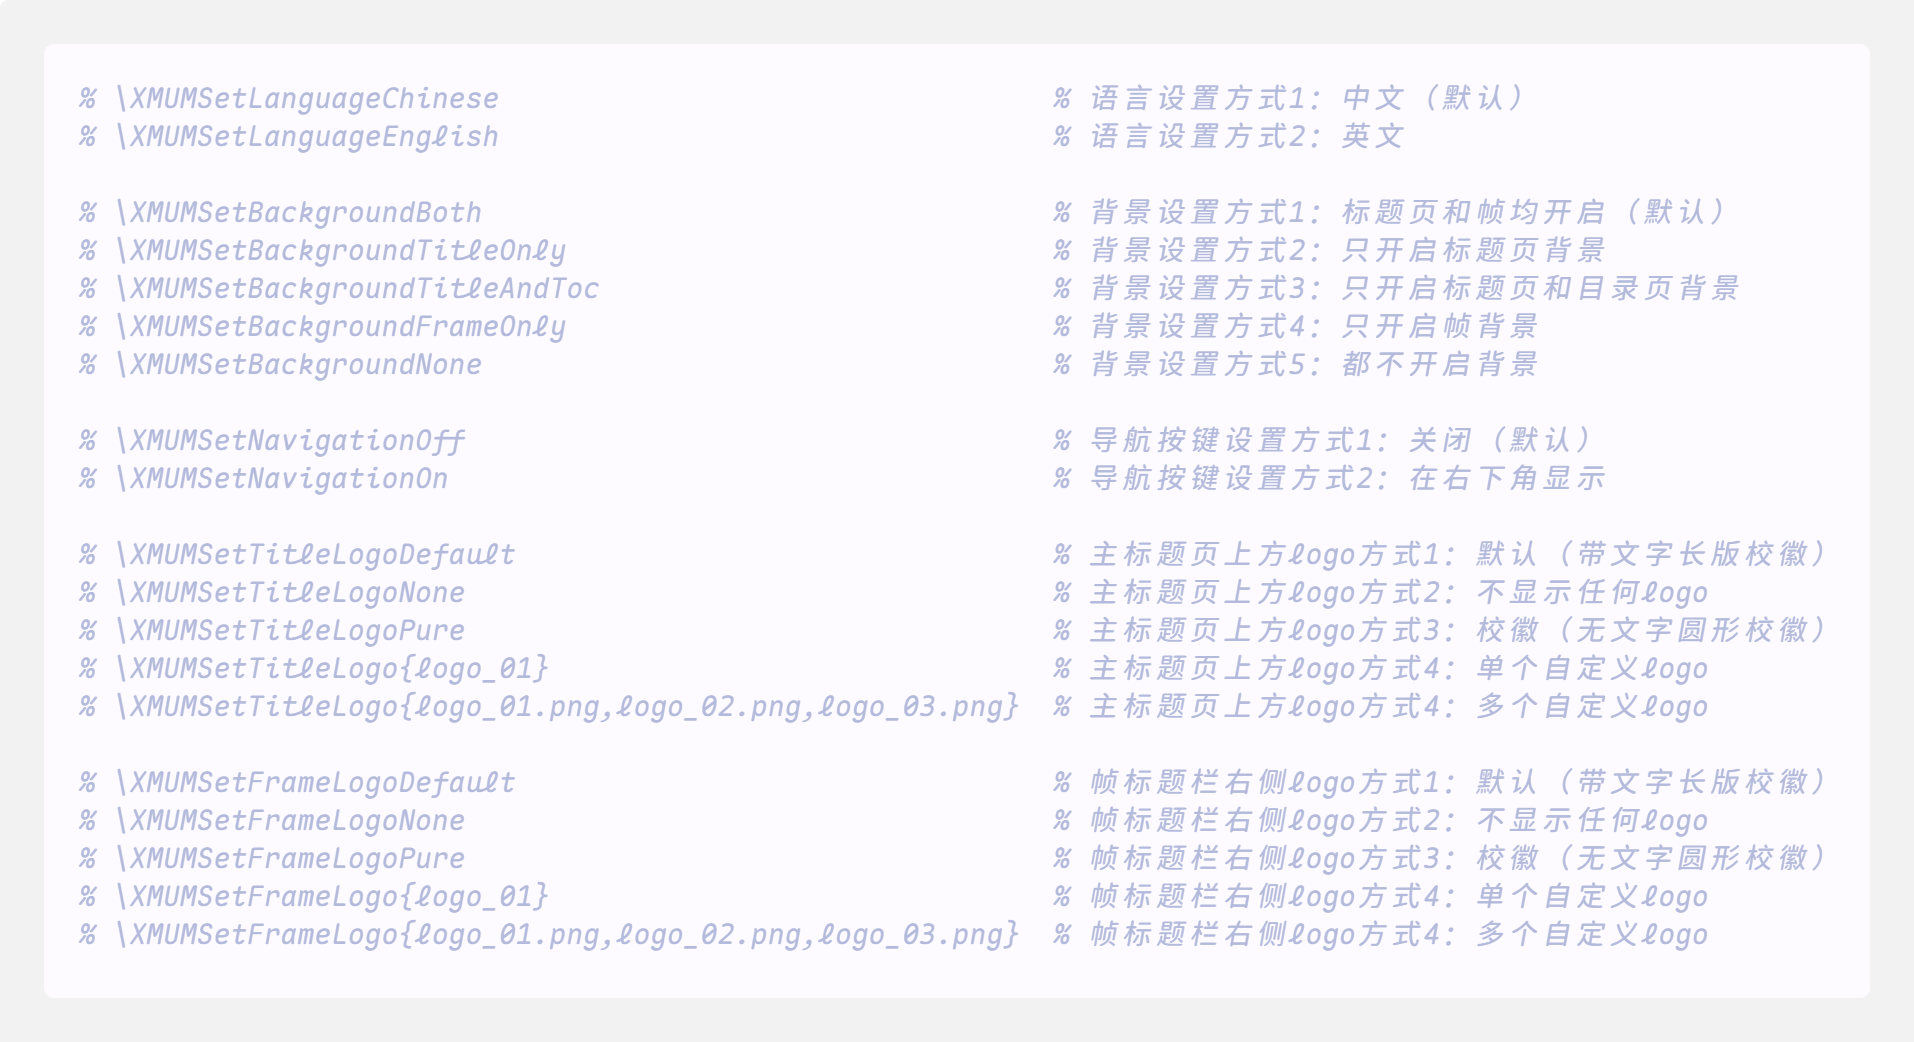
\includegraphics[width=0.72\textwidth]{img/img-1.png}
    \caption{接口调用（可取消对应位置的注释来调用该接口）}
    \end{figure}
\end{frame}

\begin{frame}[nobg]{接口示例（一）}
    \vspace{-10pt}
    \begin{columns}[T]
        \begin{column}{0.36\linewidth}
            \begin{figure}
                \centering
                
\includegraphics[width=\linewidth]{img/img-2.png}
                \caption{默认长版校徽}
            \end{figure}
        \end{column}
        \begin{column}{0.36\linewidth}
            \begin{figure}
                \centering
                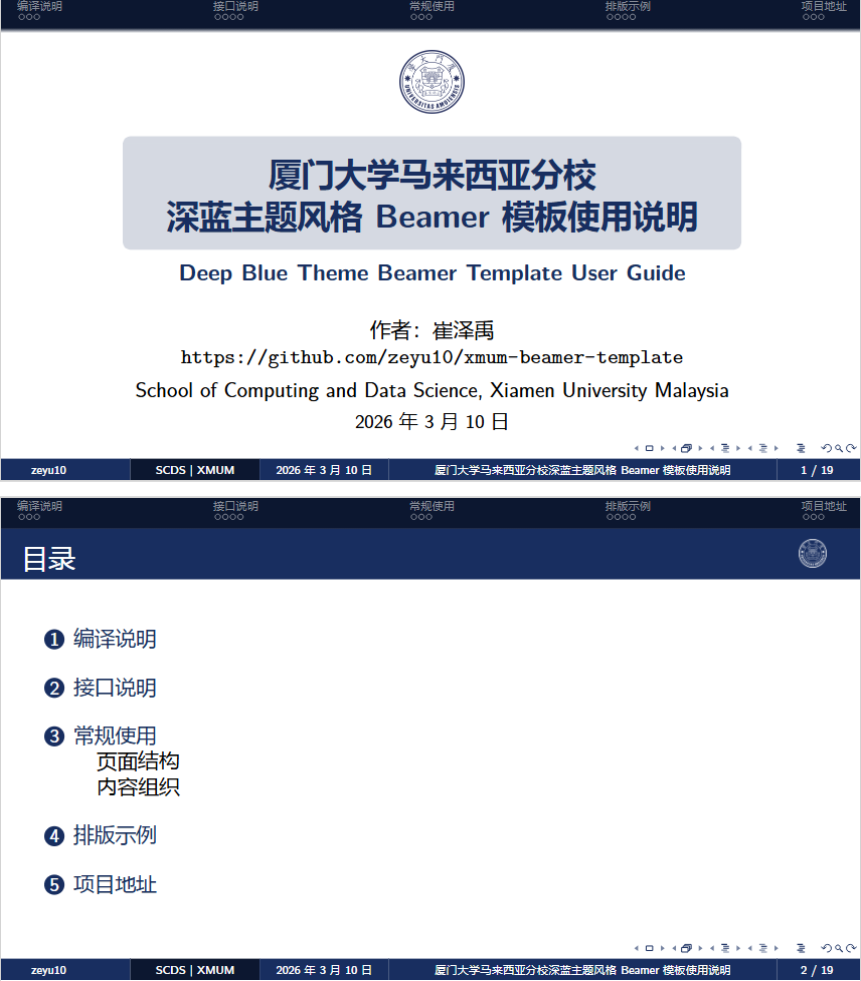
\includegraphics[width=\linewidth]{img/img-3.png}
                \caption{使用圆形校徽}
            \end{figure}
        \end{column}
    \end{columns}
\end{frame}

\begin{frame}[nobg]{接口示例（二）}
    \vspace{-10pt}
    \begin{columns}[T]
        \begin{column}{0.36\linewidth}
            \begin{figure}
                \centering
                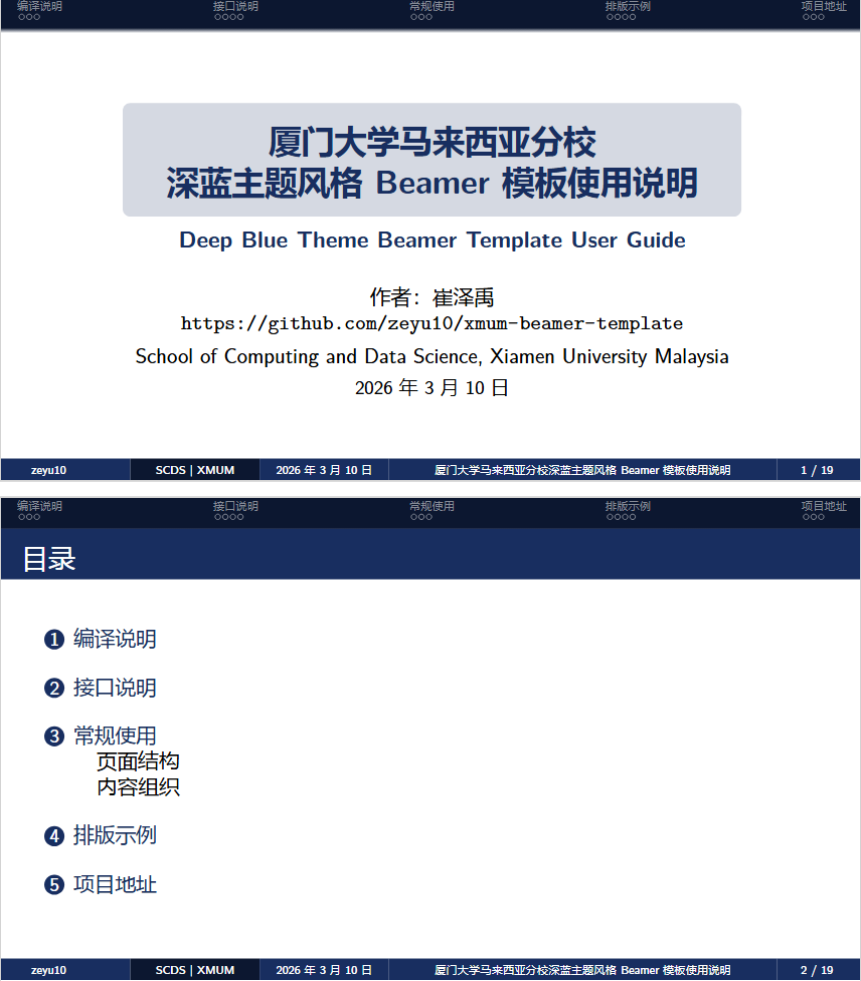
\includegraphics[width=\linewidth]{img/img-4.png}
                \caption{不显示任何 Logo}
            \end{figure}
        \end{column}
        \begin{column}{0.36\linewidth}
            \begin{figure}
                \centering
                
\includegraphics[width=\linewidth]{img/img-5.png}
                \caption{使用自定义 Logo}
            \end{figure}
        \end{column}
    \end{columns}
\end{frame}

\section{常规使用}

\subsection{页面结构}

\begin{frame}{常用文稿结构}
    \begin{enumerate}
        \item 在导言区设置标题、作者、单位、日期等元数据。
        \item 在 \texttt{\textbackslash begin\{document\}} 后调用模板接口，例如 Logo 及路径、背景、导航按键与语言设置等。
        \item 使用 \texttt{\textbackslash XMUMTitleFrame} 生成标题页，再单独放置目录页。
        \item 按内容组织为 \texttt{\textbackslash section} \texttt{\textbackslash subsection}... 以及若干 \texttt{\textbackslash begin\{frame\}\{帧标题\}} 进行内容编排。
        \item 若某一页不需要背景，可写为 \texttt{\textbackslash begin\{frame\}[nobg]\{帧标题\}} 来关闭背景。
        \item 若当前页包含 \texttt{lstlisting} 或 \texttt{verbatim} 等原样代码环境，则需将参数写为：\texttt{\textbackslash begin\{frame\}[fragile]\{帧标题\}} 或 \texttt{\textbackslash begin{frame}[fragile,nobg]\{帧标题\}}
        \item 若包含参考文献，可在末尾加入参考文献页或项目地址页。
    \end{enumerate}

    \begin{block}{建议}
        可参考 \texttt{xmum\_beamer\_readme.tex} 中的示例结构，根据实际需求进行调整。
    \end{block}
\end{frame}

\subsection{内容组织}

\begin{frame}{常见内容组织方式}
    \begin{columns}[T]
        \begin{column}{0.56\linewidth}
            \begin{itemize}[<+-| alert@+>]
                \item 使用 \texttt{itemize} 展示并列要点。
                \item 使用 \texttt{enumerate} 展示步骤、流程或阶段性安排。
                \item 使用 \texttt{subsection} 让目录和导航更清晰。
                \item 需要对比信息时，优先使用表格代替长段文字。
            \end{itemize}
        \end{column}
        \begin{column}{0.42\linewidth}
            \begin{table}
                \centering
                \scriptsize
                \begin{tabular}{ll}
                    \toprule
                    内容类型 & 推荐形式 \\
                    \midrule
                    观点总结 & 列表 \\
                    流程步骤 & 编号列表 \\
                    数据对比 & 表格 \\
                    强调内容 & 普通信息块（Block） \\
                    示例说明 & 示例信息块（ExampleBlock） \\
                    注意事项 & 提示信息块（AlertBlock） \\
                    \bottomrule
                \end{tabular}
            \end{table}
        \end{column}
    \end{columns}
\end{frame}

\section{排版示例}

\begin{frame}[nobg]{公式与列表（关闭背景示例）}
    \begin{itemize}
        \item 可直接混排中文与英文。
        \item 默认使用 \texttt{xmum\_building\_blue.png} 作为背景，且已降低透明度。
        \item 若某一页不需要背景，可写为 \texttt{\textbackslash begin\{frame\}[nobg]\{帧标题\}} 来关闭背景。
        \item 若当前页包含 \texttt{lstlisting} 或 \texttt{verbatim} 等原样代码环境，则需将参数写为：\texttt{\textbackslash begin\{frame\}[fragile]\{帧标题\}} 或 \texttt{\textbackslash begin{frame}[fragile,nobg]\{帧标题\}}
    \end{itemize}

    \begin{block}{单源最短路算法 Dijkstra 时间复杂度}
        \[
            T = O((n + m)\log n)
        \]
    \end{block}
\end{frame}

\begin{frame}[nobg]{信息块示例（关闭背景示例）}
    \vspace{-4pt}
    \begin{block}{普通信息块 \textbackslash begin\{block\}}
        \begin{itemize}
            \item 适合放置定义、结论或一般性说明。
            \item 也可用于放置算法描述、伪代码或其他需要强调的内容。
        \end{itemize}
    \end{block}
    \vspace{-4pt}
    \begin{exampleblock}{示例信息块 \textbackslash begin\{exampleblock\}}
        \begin{itemize}
            \item 适合放置具体示例、案例分析或应用场景。
            \item 也可用于放置练习题、思考题或参考写法。
        \end{itemize}
    \end{exampleblock}
    \vspace{-4pt}
    \begin{alertblock}{提示信息块 \textbackslash begin\{alertblock\}}
        \begin{itemize}
            \item 适合放置注意事项、限制条件或需要强调的内容。
            \item 也可用于放置警告信息、常见错误或重要提醒。
        \end{itemize}
    \end{alertblock}
\end{frame}

\begin{frame}[fragile,nobg]{代码快示例（关闭背景示例）}
\begin{lstlisting}
#include <bits/stdc++.h>
using namespace std;

int main() {
    cout << "Hello, World!" << endl;
    return 0;
}
\end{lstlisting}
\vspace{5pt}
\begin{alertblock}{参数说明}
    \begin{itemize}
        \item 代码环境需要使用 \texttt{fragile} 参数。
        \item 如果同时还需要关闭背景，则参数应为 \texttt{[fragile,nobg]} 来确保代码环境正常显示。
    \end{itemize}
\end{alertblock}
\end{frame}

\section{项目地址}

\begin{frame}{项目地址}
    模板地址：
    \begin{block}{GitHub}
        \url{https://github.com/zeyu10/xmum-beamer-template}
    \end{block}

    参考项目：
    \begin{block}{GitHub}
        \url{https://github.com/tuna/THU-Beamer-Theme}
    \end{block}

    \begin{block}{GitHub}
        \url{https://github.com/iceduu/xmu-beamer}
    \end{block}
\end{frame}

% \section{参考文献示例}

% \begin{frame}{参考文献示例（一）：直接在当前文件中书写}
%     本页演示在当前 tex 文件中直接引用参考文献。
%     \begin{thebibliography}{99}
%         \bibitem{knuth1984texbook}
%         Donald E. Knuth.
%         \newblock {\it The TeXbook}.
%         \newblock Addison-Wesley, 1984.
%     \end{thebibliography}
% \end{frame}

% \begin{frame}{参考文献示例（二）：引用外部 .bib 文件}
%     本页演示引用外部 .bib 文件。
%     % 使用前请先在同目录新建 refs.bib，并写入类似如下条目：
%     % @book{knuth1984texbook,
%     %   author    = {Donald E. Knuth},
%     %   title     = {The TeXbook},
%     %   publisher = {Addison-Wesley},
%     %   year      = {1984}
%     % }
%     \bibliographystyle{plain}
%     \bibliography{refs}
% \end{frame}

\begin{frame}{感谢}
    \begin{center}
        {\Large 感谢阅读和使用此模板}
    \end{center}
\end{frame}

\end{document}